\documentclass[10pt,letterpaper]{article}
\usepackage[utf8]{inputenc}
\usepackage{amsmath}
\usepackage{amsfonts}
\usepackage{amssymb}

\usepackage[margin=0.5in]{geometry}
\usepackage{graphicx}
\usepackage{booktabs}
\pagenumbering{gobble}

\title{Feature Testing}
\author{
	Cai, Zelin\\
	\and
	Silvestre, Patrick\\
}
\date{}

\begin{document}
\maketitle
\section{Calendar - Add Event as Student (Simplified Version)}
\subsection{Input Domain}
The input domain of this features includes the title of the event, a date, a starting time, a ending time, a location, and a calendar. The input domain can be partitioned: e.g. one partition for title, one partition for date, etc.

\begin{figure}[h]
	\centerline{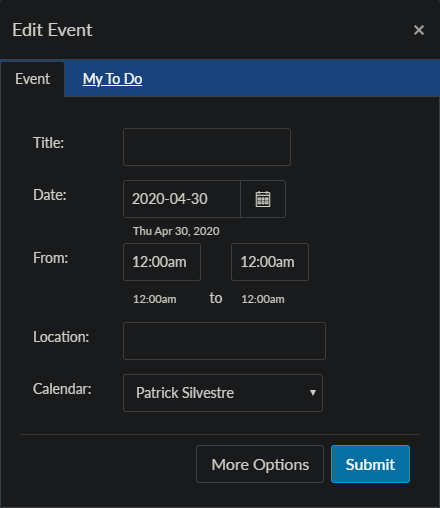
\includegraphics[width=10cm]{screenshots/edit-event.png}}
	\caption{Add Event Interface}
\end{figure}

\newpage
\subsubsection{Title}
The input domain of the input title is a string, which may be empty.

\subsubsection{Date}
The input domain of the date is a string in the format \texttt{YYYY-MM-DD}, where \texttt{YYYY} represents a year, \texttt{MM} represents a month, and \texttt{DD} represents a day. The month and day fields need not be padded with zeros. Alternatively, a user can opt to input a date using a GUI in the form of a calendar.

\subsubsection{Starting Time}
The input domain of the starting time is a string in the format \texttt{HH:MMxx}, where \texttt{HH} represents hours, \texttt{MM} represents minutes, and \texttt{xx} represents AM or PM (case insensitive). The hour and minute fields need not be padded with zeros.

\subsubsection{Ending Time}
The input domain of the ending time is a string in the format \texttt{HH:MMxx}, where \texttt{HH} represents hours, \texttt{MM} represents minutes, and \texttt{xx} represents AM or PM (case insensitive). The hour and minute fields need not be padded with zeros.

\subsubsection{Location}
The input domain of the input title is a string, which may be empty.

\subsubsection{Calendar}
The input domain of the calendar is a list of the user's calendars, of which one can be selected.

\newpage
\subsection{Test Cases}
\begin{table}[h!]
\centering
\begin{tabular}{@{}clllc@{}}
\toprule
TC \# & Input                                                                                                                                                                                               & Expected Output                                                                                                                                                                        & Actual Output                                                                                                                                                                                                            & Tess Pass/Fail \\ \midrule
1     & \begin{tabular}[c]{@{}l@{}}title: (empty)\\ date: 2020-5-2\\ starting time: 12:00am\\ ending time: 12:00am\\ location: (empty)\\ calendar: Patrick Silvestre\\ UI: press submit button\end{tabular} & \begin{tabular}[c]{@{}l@{}}Patrick Silvestre's calendar displays\\ Untitled event on 2020-5-2\\ Event has no starting nor\\ ending time (all-day event)\end{tabular}                   & See figure 2.                                                                                                                                                                                                            & Pass           \\ \midrule
2     & \begin{tabular}[c]{@{}l@{}}title: Test\\ date: 2020-5-2\\ starting time: 12:00am\\ ending time: 12:00am\\ location: Test\\ calendar: Patrick Silvestre\\ UI: press submit button\end{tabular}       & \begin{tabular}[c]{@{}l@{}}Patrick Silvestre's calendar displays\\ Test event on 2020-5-2 with Test\\ location\\ Event has no starting nor\\ ending time (all-day event)\end{tabular}  & See figure 3.                                                                                                                                                                                                            & Pass           \\ \midrule
3     & \begin{tabular}[c]{@{}l@{}}title: Test\\ date: 2020-5-2\\ starting time: 12:00pm\\ ending time: 1:00pm\\ location: Test\\ calendar: Patrick Silvestre\\ UI: press submit button\end{tabular}        & \begin{tabular}[c]{@{}l@{}}Patrick Silvestre's calendar displays\\ Test event on 2020-5-2 with Test\\ location\\ Event has starting time 12:00pm\\ and ending time 1:00pm\end{tabular} & See figure 4.                                                                                                                                                                                                            & Pass           \\ \midrule
4     & \begin{tabular}[c]{@{}l@{}}title: Test\\ date: 2020-5-2\\ starting time: 12:00am\\ ending time: 12:00am\\ location: Test\\ calendar: Patrick Silvestre\\ UI: press submit button\end{tabular}       & \begin{tabular}[c]{@{}l@{}}Patrick Silvestre's calendar displays\\ Test event on 2020-4-25 with Test\\ location\\ Event has no starting nor\\ ending time (all-day event)\end{tabular} & See figure 5.                                                                                                                                                                                                            & Pass           \\ \midrule
5     & \begin{tabular}[c]{@{}l@{}}title: Test\\ date: 2020-5-2\\ starting time: 12:00pm\\ ending time: 11:00am\\ location: Test\\ calendar: Patrick Silvestre\\ UI: press submit button\end{tabular}       & \begin{tabular}[c]{@{}l@{}}Add Event interface should warn\\ user that event ends before it starts\\ and prevent user from submitting\\ event.\end{tabular}                            & \begin{tabular}[c]{@{}l@{}}System automatically\\ adjusts either starting\\ or ending time to\\ prevent invalid\\ times with no\\ warning, implicitly\\ allowing user to\\ submit event.\\ \\ See figure 6.\end{tabular} & Fail           \\ \bottomrule
\end{tabular}
\end{table}

\newpage
\subsubsection{Actual Output Screenshots}
\begin{figure}[h]
	\centerline{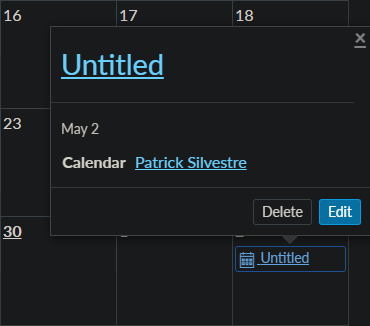
\includegraphics[width=8cm]{screenshots/tc01-actual-output.png}}
	\caption{TC-01 actual output}
\end{figure}
\begin{figure}[h]
	\centerline{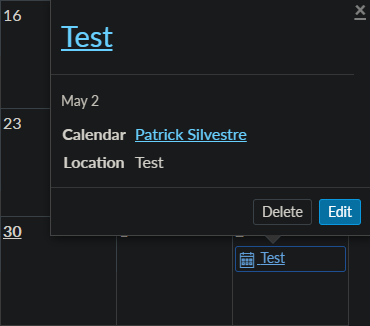
\includegraphics[width=8cm]{screenshots/tc02-actual-output.png}}
	\caption{TC-02 actual output}
\end{figure}
\begin{figure}[h]
	\centerline{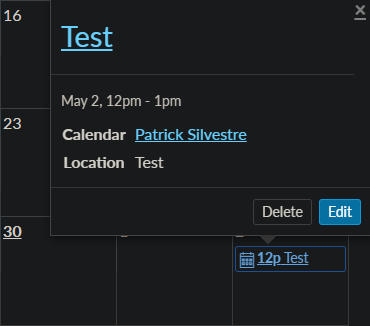
\includegraphics[width=8cm]{screenshots/tc03-actual-output.png}}
	\caption{TC-03 actual output}
\end{figure}
\begin{figure}[h]
	\centerline{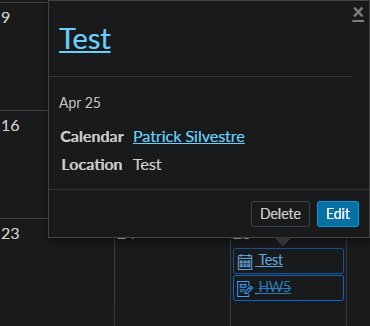
\includegraphics[width=8cm]{screenshots/tc04-actual-output.png}}
	\caption{TC-04 actual output}
\end{figure}
\begin{figure}[h]
	\centerline{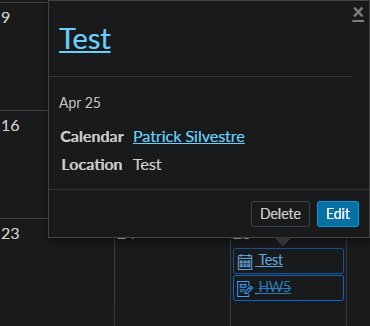
\includegraphics[width=8cm]{screenshots/tc04-actual-output.png}}
	\caption{TC-04 actual output}
\end{figure}

\end{document}